\chapter{做好准备} % Introduction chapter suppressed from the table of contents

\hypertarget{ux6211ux4eecux5f88ux6ce8ux91cdux8d28ux91cfux4e0eux5ba2ux6237ux6ee1ux610fux5ea6}{%
\subsection{我们很注重质量与客户满意度}\label{ux6211ux4eecux5f88ux6ce8ux91cdux8d28ux91cfux4e0eux5ba2ux6237ux6ee1ux610fux5ea6}}

技术总监:我们公司是一家有着光荣历史的、上规模的国有企业,除了服务于各级政府单位,还为我们集团旗下的公司提供服务,这些公司在本行业领先全国,他们也都是国有企业,所以对质量要求挺高的。\\
我:请问有什么过程改进的案例吗?\\
技术总监:我们很重视客户满意度,首先要快速解决客户的问题,同时也会组织相关团队,从过程入手查原因,比如先从配置管理看是否有问题,然后从开发测试等一层一层去查看,最终找出原因并解决,定期给高层汇报,直到客户满意。\\
我:请举些实例。\\
技术总监:因为我们的客户要求非常严格,例如他们的发文都是正式的公文,不允许有任何差错。如果因为我们的系统导致发文出现问题,作为总监,我会亲自带领团队用上面的方法分析根因,而不仅仅靠下面的团队去解决。同时,我会把问题处理的进展汇报给总经理,让他知道我们在全力以赴,争取尽快解决问题。\\
我:请问怎样监控项目?关注什么指标?\\
技术总监:每月都会与项目经理开会,主要关注项目的偏差,如进度/工作量。\\
我:为什么只关注进度/工作量偏差,你们不是也非常关注质量吗?\\
技术总监:我们也会讨论项目遇到的问题。\\
我:关于缺陷有什么统计?\\
技术总监:有的,我们会收集与分析(客户发现的)软件的缺陷数。\\
我:请问以往大概是什么水平?\\
技术总监:不太清楚,反正我们也关注。\\
我:你们不是希望从定性上升到定量管理吗?软件开发有个特点,缺陷发现得越晚返工越多,发现越早越容易解决(返工工时也小)
。。。。\\
我接下来继续与总监分析现在他们大部分缺陷还是后期才发现,导致大量返工,如果能提前发现并解决可以大大降低研发成本(不仅仅提升产品质量);正如首篇所说的,无论个人还是公司,所有改进(或创新)的前提是认识到现状与目标有差距。
从管理层关注的度量项可以反推公司会在哪方面有所改善,
如果管理层主要关注的是项目是否有延误,而不重视软件开发质量,软件开发不会有任何显著改善。

我们可以从以上故事了解到,高层都会说注重质量,但实际上不一定关注。如果要提升质量,首先要使用历史数据,画趋势图,知道自己当前的水平与范围(基线),识别异常点就可以帮公司预警,而不是应对客户投诉事件。应对投诉的根因分析属于救火。

\begin{description}
\item[]
\begin{description}
\tightlist
\item[]
= = =
\end{description}
\end{description}

根因分析能帮我们从``救火''变成``预防'',首先应利用20/80原则识别分析那类问题,针对软件开发,什么工作最花工时?

\hypertarget{ux54eaux91ccux6700ux8017ux5de5ux4f5cux91cf}{%
\subsection{哪里最耗工作量}\label{ux54eaux91ccux6700ux8017ux5de5ux4f5cux91cf}}

\framebox{%
\begin{minipage}[t]{0.97\columnwidth}\raggedright
请你按过去一年的软件开发项目,按工种占项目总工作量,从最多排到最少?

\begin{enumerate}
\tightlist
\item
  编码与代码设计
\item
  交付后的所有工作,包括维护、更新与缺陷修正
\item
  交付前的评审,静态扫描,测试与缺陷修正
\item
  项目管理与监控
\end{enumerate}\strut
\end{minipage}}

可看附件中的``开发项目工作量(成本)分布'',看你的选择与`典型'分布差多远。

软件开发项目通常最大的成本是花在找出与修正缺陷。

按专家Capers JONES 先生2012年的研究,
超过10,000功能点,计划能使用25年的大型系统,接近一半的工作量都是与找出与修正缺陷相关。

\begin{description}
\item[]
\begin{description}
\tightlist
\item[]
= = =
\end{description}
\end{description}

问软件研发总监:``通常你们的项目在哪个过程中发现的缺陷最多?''

\begin{description}
\item[]
\begin{description}
\tightlist
\item[]
超过95\% 都会说最多是在系统测试,或验收测试阶段发现\\
\end{description}
\end{description}

%\url{文件:AR1缺陷数.jpg}

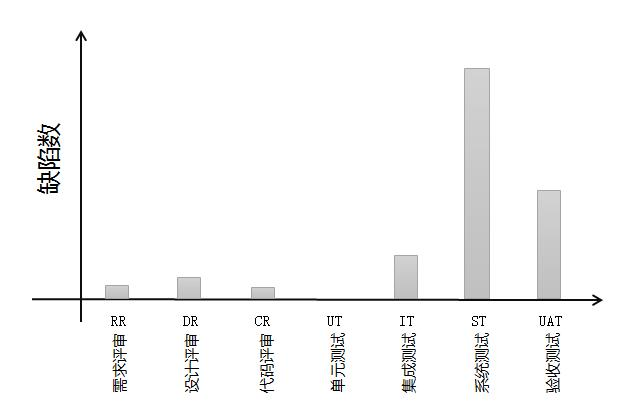
\includegraphics[width=10cm]{AR1缺陷数.jpg}

再问:用于测试与缺陷修复的返工的总工作量占整个开发项目多少?

大部分领导都没有概念。

我:如果能把后面发现的缺陷,提前在前面预先发现,估计可以节省多少工作量?

\framebox{%
\begin{minipage}[t]{0.97\columnwidth}\raggedright
当我在白板上估算出,如果能把系统测试发现的缺陷数减半,总的工作量会减少,研发成本也会降低,很多总监都会觉得不可思议,因他们一直都已经习惯了后面测试缺陷多,觉得是常态。

\begin{description}
\tightlist
\item[]
详见附件:缺陷排除率 (DRE)
\end{description}\strut
\end{minipage}}

正如质量大师Dr JURAN 强调,过程改进应从认同必须改善质量(Proof of the
Need)开始。如果大家都觉得现在的缺陷水平(例如,系统测试超过200个缺陷)是常态,任何公司级质量改进计划都不会有好结果。\\
但如果管理层了解现在未能尽早发现并排除缺陷是最好的改进方向(80/20原则),并开始重视,但应如何开始?\\
``如何能收集到修复缺陷相关工时数据?因没有度量,便无法谈改进。我们现在只有缺陷数据,与测试工作量数据。''\\
收集软件开发数据不容易,但如果没有收集到可信的数据,便无从分析与改进。\\
是否可以靠组织级加强这方面相关的度量与监控?我们先看看一家几千人的大公司,他们一直都很强调量化管理,收集各种项目的系数,度量并分析。\\

\hypertarget{ux81eaux52a8ux5316ux7edfux8ba1ux5206ux6790}{%
\subsection{自动化统计分析}\label{ux81eaux52a8ux5316ux7edfux8ba1ux5206ux6790}}

客户:我们每次都跑全量,公司引入低码平台,更多的是在需求设计阶段做好质量保证,
所以我们很注重量化质量管理,能否通过自动化来统计分析?
如何通过量化或工具方式实现自动评审?

我:为什么要自动化?

客户:从去年开始我们搞度量分析, 发现员工就会造数据, 结果导致失真,
度量哪里就造哪里,
所以还是想通过工具代替人工方式,除了能提升效率,也能帮助判断数据是否合理。\\
现在我们的主管很反感度量,一度量就有人造数据

我:度量本来是件好事

客户:是的,就是大家知道算法原理就开始造假。 因为我们搞了红黑榜,
但很多人头脑都很聪明,会想办法,但用于不合适的地方。

我们有很多数据统计分析,比如看测试用例与需求的比例。
其实客户发现的缺陷比例也降低了,但因为我们这行对质量特别注重,产品经过多年的逐步演化,过程很复杂,导致软件缺陷的修复很耗时,客户不太满意。
而且公司要求交付的频率要比以前高了很多,我们团队做这些分析都忙不过来,所以需要员工设自动化工具等加快速度才可以。\\
让我给你看看我们大数据分析。。。

我:等等,但我们首要解决如何能收集到真正的数据,不然数据分析没有意义。

客户:好的,有什么建议?

我:还记得我们上次交流,要让团队自主,不能单靠标准过程并用指标监控执行情况?

%\href{文件:Diagram_2.0.png}{500px}

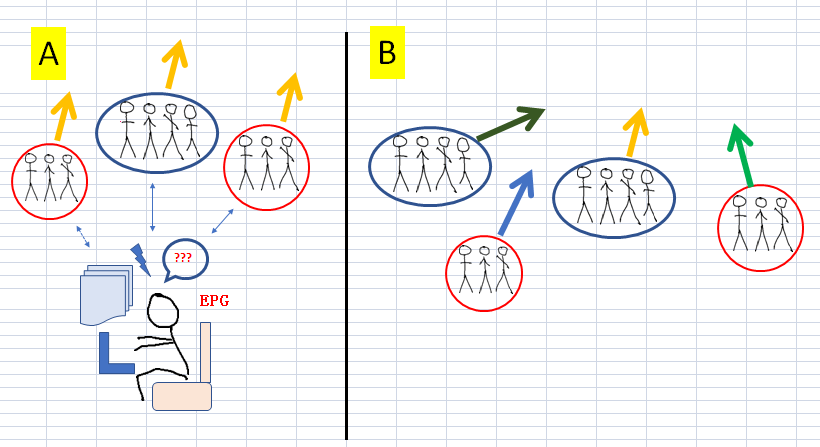
\includegraphics[width=10cm]{Diagram20.png}

我:请问你们是采用左面还是右面的方法做过程改进?\\
客户:好像我们现在度量分析是采用你图里左面的方法。

我:是的。总体分析还有另一不足:各个项目特性不一样,你们现在几十个项目总体趋势分析,
很可能找不对根因,因每个项目的问题(根本原因)很可能不同。
比如,同样是一个测试用例比例数,你的范围就很宽 -
从最低的0.3到最高的超过200!但你们取平均值5.1 来做分析。

收集数据也是问题,因收集数据是挺花精力的工作

客户:完全同意

我:但正因为不同项目有各种特性,要对收集到的数据做分析也很耗时。
这些辛辛苦苦做出来的分析报告其实不仅仅是给高层(或者项目经理),
在每一个团队成员都看到才有意义
。(度量分析要反馈回数据提供者,他们才有动力继续收集数据)要把那些分析好的报告再跟每一个团队成员解释上要花多大精力?

\textbf{度量的主要目的是从数据分析找出根因做改进而不是仅仅为了监控}

如果把数据分析下放到团队自己搞,便灵活多了;也正因为他们有参与收集和分析讨论,
你们也可以节省很多沟通的成本。

所以你们领导应该定位自己是内部老师,辅导团队怎么做好数据分析,效果会更好。

客户:就当团队自己讨论便可以得到改进吗?不需要我们领导?\\
我:
如果团队有能力,应该放手让他们自己利用收集数据,分析做改进。你们管理者应从以前分析数据,定位为团队的教练,辅导他们。千万不要误以为比以前自己做分析轻松,你们须要更熟悉,但因你们之前有经验,所以辅导团队应不会太难。更大的挑战反而是要管理层了解并赞同敏捷开发的团队自主思路。

\hypertarget{ux603bux7ed3}{%
\subsubsection{总结}\label{ux603bux7ed3}}

\begin{itemize}
\tightlist
\item
  为了确保质量应该用精益的概念。每一小步确认限制级,确保达标。然后与客户确认,而不是先定一个总体的几个月计划。按总计划监控任务是否延误?因为后者会把团队的关注点都放到按时交付去,无法确保最终的产品达到高质量要求
\end{itemize}

\begin{itemize}
\tightlist
\item
  如果要从救火的管理思路变为基于找出根本原因预防问题发生的思路,就需要在每次冲刺迭代后依据数据,团队一起分析根因并制定解决措施
\end{itemize}

\begin{itemize}
\tightlist
\item
  若要改进行动有效,就不应单靠从上而下推的管理,必须让团队参与
\end{itemize}

\hypertarget{ux9644ux4ef6}{%
\section{附件}\label{ux9644ux4ef6}}

\hypertarget{ux516cux53f8ux9ad8ux5c42ux4e0dux4e00ux5b9aux5173ux6ce8ux8d28ux91cf}{%
\subsection{公司高层不一定关注质量}\label{ux516cux53f8ux9ad8ux5c42ux4e0dux4e00ux5b9aux5173ux6ce8ux8d28ux91cf}}

\framebox{%
\begin{minipage}[t]{0.97\columnwidth}\raggedright
问:在传统 IT的公司,无论是 Bug
率还是其他质量指标对业务的影响的相关性都不容易度量,只有重大事件才会让公司在客户面前失去信任,所以高层不会真正的重视质量。\\
答:理解,但软件BUG的暴露越往后,返工的工作量就越高,而且是几何级数的增加(例如在单元测试或评审发现都可以1人时内解决;系统测试通常要花起码20人时,客户使用后才发现便更高)。但在很多IT公司,大部分缺陷都是在系统测试、甚至到验收测试才发现。如果能把软件缺陷的发现前移,把通过系统测试、验收测试发现的缺陷减半,便可以大量降低质量成本,提升开发生产率。所以我建议上面北京公司的质量总监利用缺陷数估算返工的工作量来引起老板重视。(而不是仅仅说降低缺陷率)\\
问:有些业务客户可能不一定关注缺陷密度。举例:有些互联网公司关注系统的高可用性(按电信标准的99.99\%可用),因为高可用性会给业务上带来稳定的广告展现机会,也就是广告的库存。他们也关注上线后低异退率(如,上线后异退率:3/万,异退是各种复杂原因的异常退出),异退会对用户流失产生正相关的影响。\\
答:系统的可用性,异退率等指标,也是可以连续收集到的(如,每天、每周),同样可以用上面深圳企业的方法,画控制图,预警过程有没有异常变动,如有异常便要启动根因分析,找到过程异常的根因,避免等到客户投诉才救火。\\
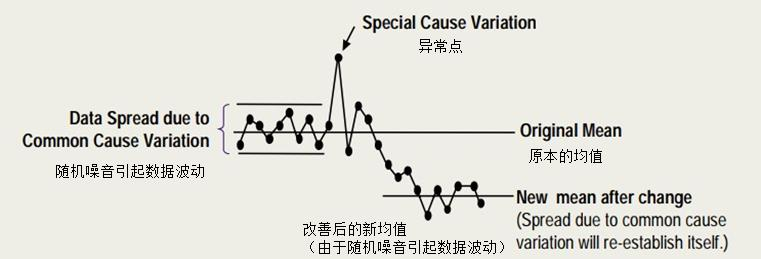
\includegraphics[width=10cm]{MGR_f11.jpg}
\strut
\end{minipage}}

%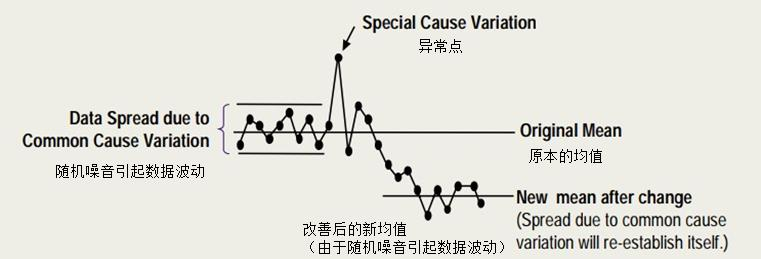
\includegraphics[width=10cm]{MGR_f11.jpg}

\hypertarget{ux8d28ux91cfux6210ux672c-coq-cost-of-quality}{%
\subsection{质量成本 COQ (Cost of
Quality)}\label{ux8d28ux91cfux6210ux672c-coq-cost-of-quality}}

质量成本由三部分组成:

\begin{enumerate}
\tightlist
\item
  失效(Failure)成本\\
  把缺陷修复好的成本,包括在客户现场被发现的缺陷。
\item
  评测(Appraisal)成本\\
  包括各类测试,如系统测试,集成测试,单元测试等,所花的工时
\item
  预防(Prevention)成本\\
  包括技术评审 (注:有些人把评审归为评测成本,这里按 Mr.Juran
  定义,归属于预防成本)
\end{enumerate}

如变通理解以上COQ定义,``如何通过提高评审效率来降低质量成本``便可对应COQ各部分:\\
失效(Failure)成本:原本所有与缺陷相关的成本\\
评测(Appraisal)成本:增加测试前的静态扫描、评审,减少失效(Failure)成本,使总COQ下降\\
预防(Prevention)成本:减小缺陷的产生,例如用原型做好需求,进一步使总COQ下降\\

\hypertarget{ux7f3aux9677ux6392ux9664ux7387-dre}{%
\subsection{缺陷排除率 (DRE)}\label{ux7f3aux9677ux6392ux9664ux7387-dre}}

%\href{文件:jalote_emm_7.1_1.0.png}{500px}

\includegraphics[width=10cm]{jaloteemm7110.png}

Figure7.1,从需求到设计、编码、单元测试、系统测试、验收,整个开发过程大家都很熟悉(缺陷只会源自需求、设计、编码);需求、设计、编码后都会评审/测试来排除缺陷,但仅仅做评审/测试不一定能确保质量。因为最终验收缺陷数取决于每个步骤能否有效排除当前的缺陷。

所以可以用缺陷排除率(Defect Removal Efficiency DRE)
来衡量测试或评审的效率:

%\href{文件:Ma3_1.0.png}{文件:Ma3 1.0.png}

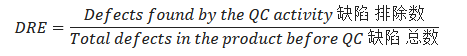
\includegraphics[width=10cm]{Ma310.png}

缺陷排除率除了可以用于整个项目,包括测试,也可以用于前面评审、扫描等。

\begin{description}
\item[]
\begin{description}
\tightlist
\item[]
= = =
\end{description}
\end{description}

有些人会认为尽早发现并解决缺陷
对质量肯定好,但会耗费工作量,增加项目成本,老板不一定愿意。
其实是反过来,如能在前面预先发现并修正缺陷,
便能减小后面测试和修改缺陷的工作量, 最终只会减少总项目工作量。

%\href{文件:AR1FixVarCostScreenshot_2022-12-10_144400.jpg}{600px}

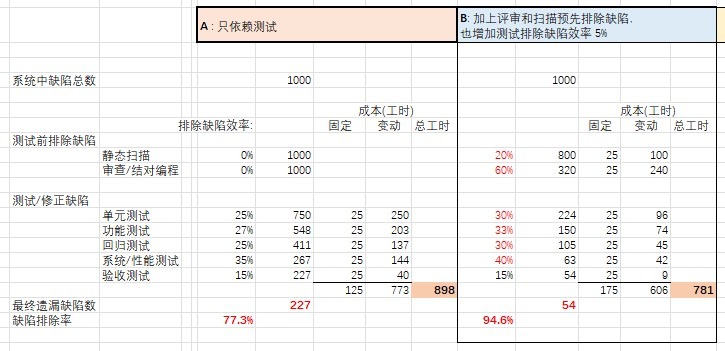
\includegraphics[width=10cm]{AR1FixVarCostScreenshot20221210144400.jpg}

比较以上两种策略的质量成本(COQ)就能看出:

\begin{itemize}
\tightlist
\item
  增加测试前扫描与审查,并加大测试效率,不仅减少最终缺陷数到54(对比227),也降低总质量成本(总人时)
\end{itemize}

\framebox{%
\begin{minipage}[t]{0.97\columnwidth}\raggedright
假设:每项任务的固定成本都是25人时;测试前的缺陷修复:每缺陷用 0.5人时;测试缺陷修复,上面计算假定每缺陷用1人时,详见下表: \\
\begin{tabular}{|c|c|c}\hline
\multicolumn{2}{c}{\mbox{每缺陷修正工时}}\\ \hline
\mbox{扫描/评审}&0.5 \\ \hline
\mbox{单元/功能测试}&1 \\ \hline
\mbox{系统/性能测试}&1 \\ \hline
\mbox{验收测试}&1 \\ \hline


\end{tabular}
通常测试里的缺陷修复每缺陷不只一人时,例如,在验收阶段时可能要用20人时;我通常会打开这XLS
表,填上客户的估计值。从上表看到,即使用最少的1人时来算,还是不亏。

\strut
\end{minipage}}



因为缺陷已经提前被排除系统测试的缺陷减少,测试阶段的工作量减少大于前面扫描评审上的投入。

可以进一步利用COQ概念,增加早期预防缺陷措施,如用原型与客户交流,做好需求调研,进一步减少缺陷,和成本。
例如,使用原型与场景与客户挖掘需求,可进一步把缺陷降到43,也降低总质量成本:

%\href{文件:est缺陷表3.jpg}{600px}

\includegraphics[width=10cm]{est缺陷表3.jpg}

\texttt{注:你可能会质疑使用原型方法不只25人时,但即使加大到100人时,还是不亏。因它能预防缺陷,整体缺陷数下降20\%,使总质量成本下降超过100人时。}

\hypertarget{ux5f00ux53d1ux9879ux76eeux5de5ux4f5cux91cfux6210ux672cux5206ux5e03}{%
\subsection{开发项目工作量(成本)分布}\label{ux5f00ux53d1ux9879ux76eeux5de5ux4f5cux91cfux6210ux672cux5206ux5e03}}

参考Capers JONES先生 2012 的例子,汇总成以下比例:

%\url{文件:AR1成本占比.jpg}

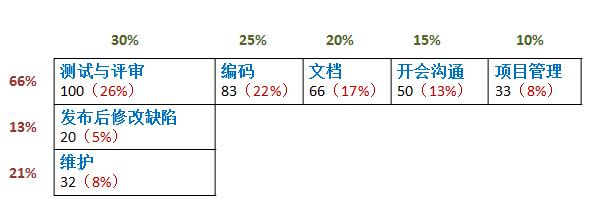
\includegraphics[width=10cm]{AR1成本占比.jpg}

测试与评审一般占开发工作量的30\%

测试与评审一般占总质量成本(包括发布后维护与改缺陷工作)的66\%

把所有工作量都加起来,测试与评审还是占最大(26\%) , 编码第二 (22\%)

\framebox{%
\begin{minipage}[t]{0.97\columnwidth}\raggedright
注意:`测试与评审`包括所有与缺陷相关的成本,包括单元测试、静态扫描、
评审与相关的缺陷修正, 而编码只包括设计与编写代码部分。
例如,有些人会觉得比例应该是:\\
开发30\%,测试和bug修改25\%,需求和设计20\%,项目管理和沟通20\%,文档5\%

但如果按上面的定义,开发部分很可能已包括单元测试、静态扫描与改正缺陷工作,
如把这些都归到测试评审里会变回类似上图的比例。\strut
\end{minipage}}

\hypertarget{reference}{%
\section{Reference}\label{reference}}

1. Jones, Capers: "Software Quality Metrics: Three Harmful Metrics and
Two Helpful Metrics" 2012.\\
